\subsection{Softwarequalität}
Hier finden sich die Neuerungen zum Thema Infrastruktur

\subsubsection{Qualitätssicherung der Oberfläche}
Am Ende des Entwicklungsprozesses wurde die Oberfläche noch nach Problemen in der Darstellung der Assets oder nach Rechtschreibfehler geprüft. Gegebenenfalls wurden die Rechtschreibfehler korrigiert, Positionierungsfehler angepasst, Assets neu erstellt und eingebunden oder vergessene Kantenglättungen hinzugefügt. 
\begin{itemize}
\item 934a8aed1a360ca2e1d56001e67cafcde8abcaa5
\item cd8e1d9aea24ffe4f4cf9d8d9330813135fffd33
\item 59e936934a9056a776462f07bc45005943dd2121
\item 749b75fc52b7a87f67cf4e1256359747d0f37ed3
\end{itemize}

\subsubsection{Unit-Tests}
Im letzten Semester entschied sich das Projektteam dafür, Unit-Tests als einen Baustein zur Absicherung der Software-Qualität einzusetzen. Hierzu wurden relativ einfache Unit-Tests mit JUnit implementiert. Dies erfolgte leider verhältnismäßig spät, als die Code-Basis bereits komplexer war. Hierbei wurde jedoch festgestellt, dass sich einfache Model-Klassen wie "Deck" sehr einfach und isoliert testen liesen, jedoch komplexere Klassen wie der "BattleController" nur mit erheblichen Aufwand. Das mocken dieses Controllers, der die zentralen Spielmechaniken steuert, stellte sich als größeres Problem heraus. Verschiedene versuche diesen separiert vom laufenden Projekt zu instanzieren und zu testen schlugen fehl, da die entsprechenden LibGDX-Dependencies ohne laufendes Projekt fehlten. Bei einer ersten Recherche, stießen wir auf die Option die entsprechenden Komponenten mittels dem Framework "Mockito" zu simulieren - das Team entschied sich jedoch aufgrund des hierfür nötigen Aufwands dafür, die Software-Qualität über den zentralen Abnahme-Prozess der Branches sowie die Prüfung von Metriken und manuellen Tests herzustellen. \\
Hier exemplarisch ein Test für das Gameobject "Deck":
\begin{lstlisting}
    @Test
    void getSize() {
        assertTrue(deck.getSize() > 0);
    }
\end{lstlisting}
Vorab wird ein Deck deklariert und in diesem Test die getSize()-Methode geprüft, ob diese valide Ergebnisse zurück gibt. Abschließend lässt sich sagen, dass Unit-Tests ein elementarer Baustein unserers Software-Qualitäts-Konzepts waren und diese kaum umgesetzt wurden. 

\subsubsection{Metriken}
Zur Analyse wurden verschiedene Tools herangezogen. Zur Auswahl standen: "PMD" und "Metrics Reloaded". Für beide liegt ein IntelliJ-Plugin vor, was die Einbindung in unser Projekt deutlich erleichterte. Beide Tools hatten entsprechend ihre Vor- und Nachteile, die hier kurz erörtert werden sollen.
\textbf{PMD}
PMD bietet diverse Optionen zur konkreten Code-Analyse. Dabei lässt sich nach verschiedenen "Verstößen" z. B. gegen Best Practices suchen und diese ggf. korrigieren. PMD liefert die Ergebnisse dabei in einer Art Baumstruktur und referenziert betroffene Stellen direkt im Code, sodass Änderungen einfach vorgenommen werden können. PMD liefert damit bei entsprechendem Fachwissen solide Ergebnisse über Schwachstellen unserer Software. Für einen einfachen Einsatz um einen Überblick über Problemstellen zu erhalten ist PMD jedoch potentiell zu komplex. 
Hier ein Auszug der umfangreichen Findings mit PMD:
\begin{figure}
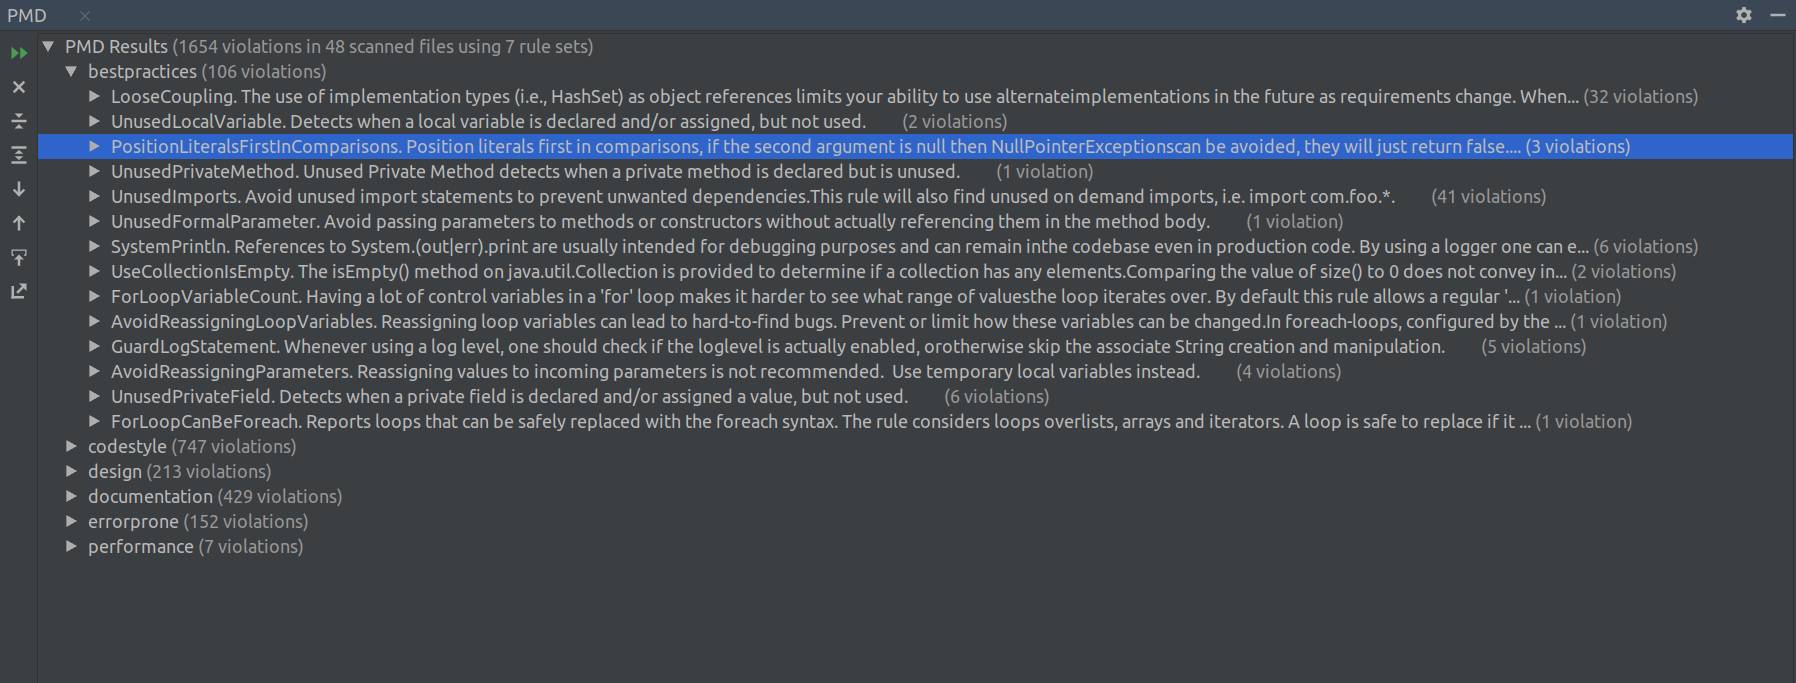
\includegraphics[width=1\textwidth]{../img/sq/pmd1.PNG}
\caption{Screenshot: PMD Übersicht}
\label{fig:Screenshot PMD Übersicht}
\end{figure}
Beispielsweise lässt sich hier sehr einfach feststellen, dass es eine konkrete Implementation gibt die ggf. gegen Loose Coupling verstößt, was spätere Änderungen ggf. erschwert da ein höherer Grad an Abhängigkeit implementiert wurde als vielleicht notwendig. 
\begin{figure}
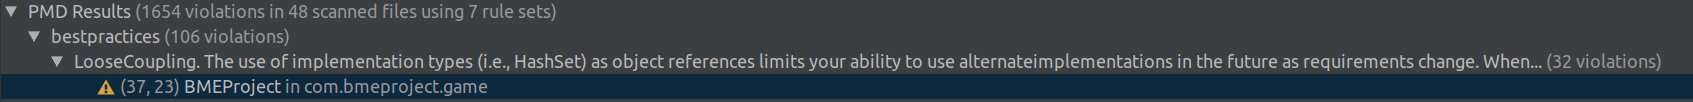
\includegraphics[width=1\textwidth]{../img/sq/pmd2.PNG}
\caption{Screenshot: PMD Beispiel}
\label{fig:Screenshot PMD Beispiel}
\end{figure}
In Abbildung \ref{fig:Screenshot PMD Beispiel} lässt sich nun das konkrete Finding adressieren und direkt im Quellcode öffnen. Konkret handelt es sich um folgende Zeile:
\begin{lstlisting}
	public static HashMap<Integer, Card> allCards;
\end{lstlisting}
Hier hätte vorzugsweise gegen das Interface "Map" implementiert werden können:
\begin{lstlisting}
	public static Map<Integer, Card> allCards;
\end{lstlisting}
Um diese Abhängigkeit aufzulösen.
\textbf{Metrics-Reloaded}
Metrics-Reloaded stellte sich für den Einstieg als bessere Option heraus. Es liefert zur Auswertung einen vollständigen HTML-Export, der mittels JavaScript eine konfigurierbare UI zur Verfügung stellt. Gleichzeitig liefert Metrics-Reloaded einfache Einschätzungen und Erläuterungen zu verschiedenen Metriken. Das machte es für uns leichter Problemstellen zu iidentifizieren und genauer zu prüfen und einen Überblick zu erhalten.\\
Beispielhaft ein Auszug eines Exports:
\begin{figure}[h]
\centering
 \subfloat[Metricsreloaded 1]{{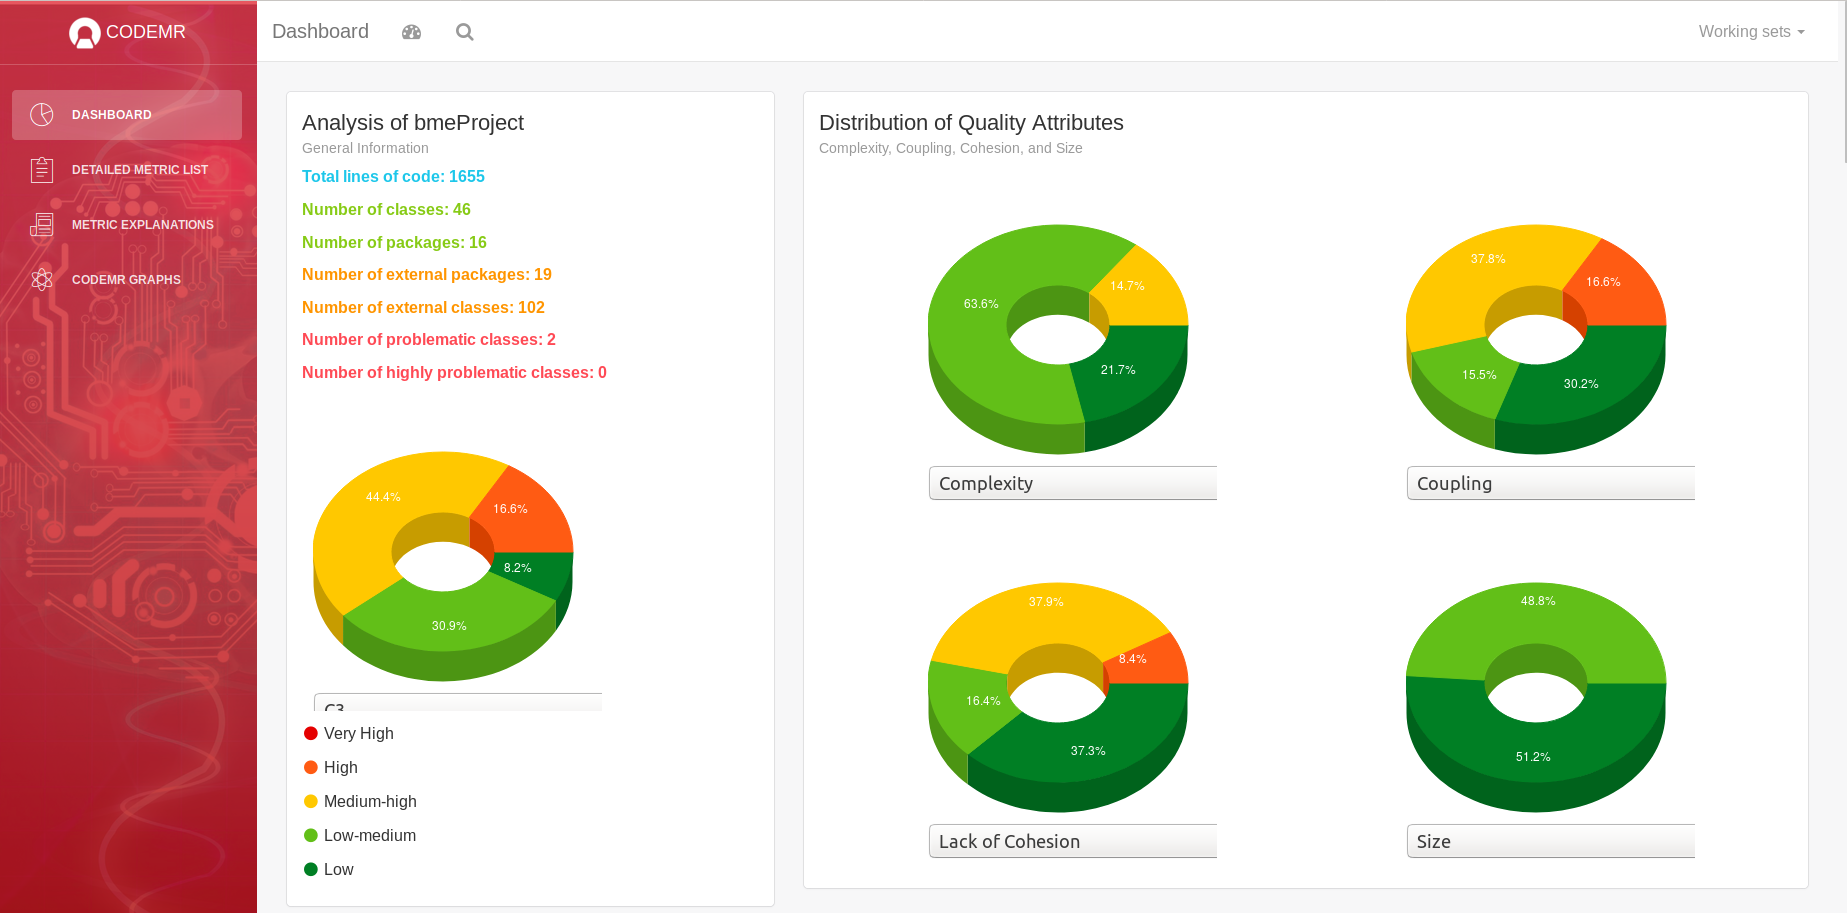
\includegraphics[width=8cm]{../img/sq/metricsreloaded1.PNG} }}
\qquad
 \subfloat[Metricsreloaded 2]{{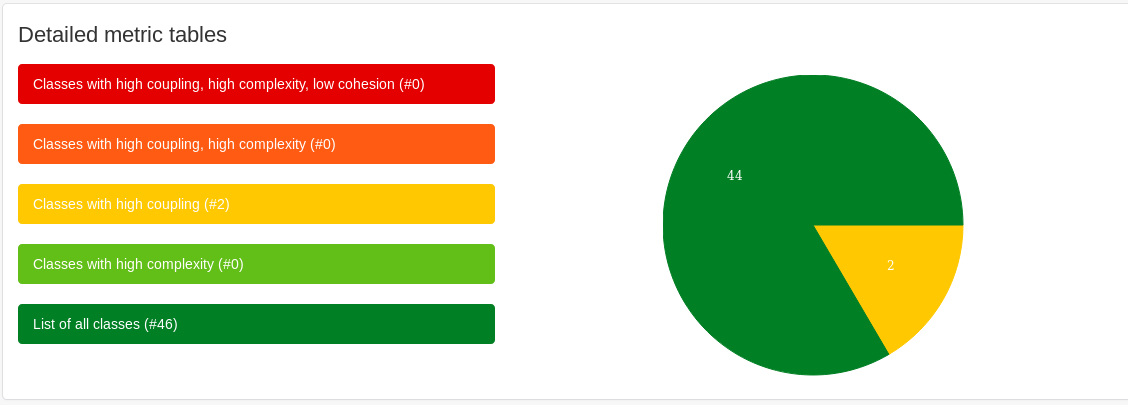
\includegraphics[width=8cm]{../img/sq/metricsreloaded2.PNG} }}
\caption{Screenshot: Metricsreloaded Überblick}%
 \label{fig: Screenshot Metricsreloaded Überblick}%
\end{figure}
In der Abbildung \ref{fig: Screenshot Metricsreloaded Überblick} lässt sich schnell erkennen, dass es zwei problematische Klassen gibt, die zu analysieren sind.
Wertet man dies nun weiter aus, erhält man die konkreten Klassen:
\begin{figure}
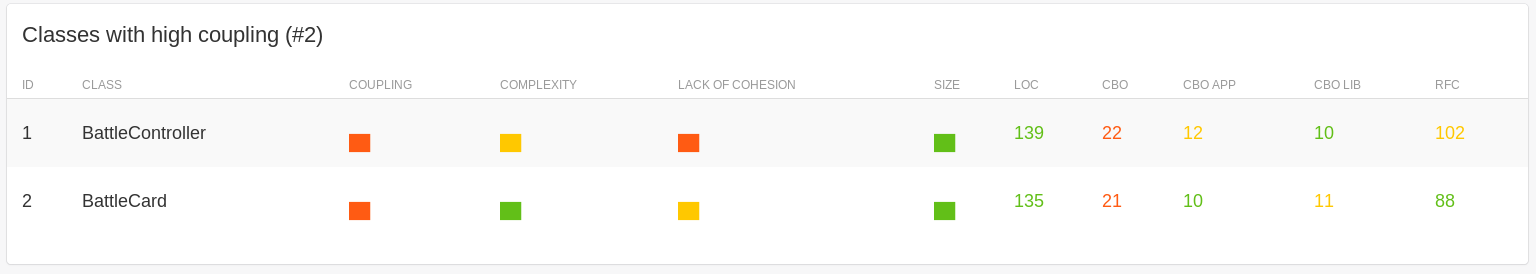
\includegraphics[width=1\textwidth]{../img/sq/metricsreloaded3.PNG}
\caption{Screenshot: Metricsreloadedl High Coupling}
\label{fig:Screenshot Metricsreloaded High Coupling}
\end{figure}
Erwartungsgemäß werden die Klassen "BattleController" und "BattleCard" als potentiell problematisch erkannt. Erwartungsgemäß deshalb, da es sich um die zwei zentralen Klassen handelt, die die Spiellogik steuern und alle Objekte in diesem Zusammenhang halten und verwalten. 

\subsubsection{Manuelle Tests}
Wie bereits unter \ref{Merging und Abnahme} angeführt, wurden unsere Feature-Branches und der nach dem Merge gebildeter neuer Stand immer manuell getestet. Hierfür besprachen wir die Anforderungen, die dieser Branch erfüllen sollte bzw. prüften diese in den jeweiligen Issues im Glo-Board und prüften daraufhin die Funktionalität manuell ab. Zusätzlich wurden hier auch ggf. Fehleingaben oder mögliche Szenarien geprüft, die als Konsequenz auftreten konnten, wie z. B. "Wird eine Null-Prüfung auf das Kartendeck durchgeführt, wenn alle Karten aufgezogen sind?". Gleichzeitig prüften wir zudem immer oberflächlich alle anderen Funktionalitäten ab, die ggf. auch unberührt von der neuen Änderung waren um Wechselwirkungen auszuschließen. 

\subsubsection{Pair-Programming und Debugging}
Pair-Programming (und in unserem Fall oft "Pair-Debugging") ist eine praktikable Methodik um die Code-Qualität zu verbessern. Gleichzeitig ist es ein nützliches Anleitungsinstrument um neuere Entwickler in ein Projekt einzuweisen.
Wie im Abschnitt \ref{Implementationen} bereits erschließen lässt, vergaben wir im Team häufig Aufgaben an mehr als eine Person auf einmal um diese gemeinsam an einer Anforderung entwickeln zu lassen. Gleichzeitig nutzten wir dies um z. B. auf unseren Team-Meetings oder Coding-Treffen gemeinsam zu programmieren und unseren Code zu debuggen. Hierbei stellten wir immer wieder fest, dass gerade komplexe Implementationen deutlich leichter umgesetzt werden können, wenn man diese einem anderen Mitglied im Prozess permanent erläutert und die logischen Operationen nochmals laut ausspricht. 

